\chapter{Lattice Gauge Theory} \label{chap::lattice_gauge_thy}

%%%%%%%%%%%%%%%%%%%%%%%%%%%%%%%%%%%%%%%%%%%%%%%%%%%%%%%%%
%%%%%%%%%%%%%%%%%%%%%%%%%%%%%%%%%%%%%%%%%%%%%%%%%%%%%%%%%
%%%%%%%%%%%%%%%%%%%%%%%%%%%%%%%%%%%%%%%%%%%%%%%%%%%%%%%%%
%lattice
The properties of hadrons constructed from strongly interacting quarks and gluons should be calculable within the relevant gauge field theory, Quantum Chromodynamics (QCD). At the energy scale of hadrons, QCD does not have a small coupling constant and must be treated non-perturbatively. The tool we will use to achieve this is lattice QCD, in which the field theory is discretized on a finite grid of Euclidean space-time points, and where we can compute correlation functions as an average over a finite but large number of possible gauge-field configurations. 
%In this chapter we will explore the gauge theory, QCD, and show how one can formulate the theory onto a discrete set of space-time points, which when coupled with an analytic continuation of time, allows for the calculation of observables. 

%%%%%%%%%%%%%%%%%%%%%%%%%%%%%%%%%%%%%%%%%%%%%%%%%%%%%%%%%
%%%%%%%%%%%%%%%%%%%%%%%%%%%%%%%%%%%%%%%%%%%%%%%%%%%%%%%%%
%%%%%%%%%%%%%%%%%%%%%%%%%%%%%%%%%%%%%%%%%%%%%%%%%%%%%%%%%

\section{The Path Integral  } \label{QCD::path_integral}
The functional integral formalism underpins modern understanding of quantum field theory. It was originally introduced by Feynman in the context of quantum mechanics, later gaining widespread use in quantum field theory. Here we sketch the basics of the path integral approach used to simulate QCD.  We will work in natural units in which $\hbar = c = 1$.  

%Throughout this section we will follow the traditional \emph{physics style} mathematics in which we use words like ``function" and ``eigenstate" improperly, exchange the order of limits, and commute integrals without consideration for the deeper mathematical issues in the interest of skipping technical details that would obscure the physical understanding. 

The two most fundamental objects we will be working with are the QCD Lagrangian, $\mathcal{L}_{\mathrm{QCD}}$, and the generating functional, $\mathcal{Z}_{\mathrm{QCD}}$. The Minkowski Lagrangian is

\begin{equation}
\mathcal{L}_{\mathrm{QCD}} = \bar{\psi}\left[i \gamma_\mu \partial^\mu - m\right]\psi + g  A_\mu^a\bar{\psi}\gamma^\mu t_a\psi - \frac{1}{4}G_{\mu\nu}^aG^{\mu\nu}_a.
\end{equation}

The quark fields, denoted by $\psi^\alpha_i(x)$,  are color-spinor fields which are functions of the space-time coordinate, $x$, with a $SU(3)$ color index $i=1,2,3$ and a Dirac spinor index $\alpha=0,1,2,3$. The quark fields transform locally\footnote{Under a gauge transformation the quark field transforms as $\psi^\alpha_i(x) \rightarrow \mathcal{G}_{ij}(x)\psi^\alpha_j(x)$, where $\mathcal{G}_{ij}(x)$ is an element of $SU(3)$ representing the gauge transformation at space-time point $x$.} under $SU(3)$ color gauge rotations while the Lagrange density is a \emph{gauge invariant} scalar density. 

The gluon fields, $A_\mu^a$, transform as Lorentz vectors and have a color index $a=1-8$ corresponding to the adjoint representation of $SU(3)$ while the $t^a$ are the generators of the gauge group, one possible basis being the Gell-Mann matrices. 

The $\gamma_\mu$ are Dirac matrices and in \emph{Minkowski} space obey the anti-commutation relation $\{\gamma_\mu,\gamma_\nu\} \equiv \gamma_\mu\gamma_\nu - \gamma_\nu\gamma_\mu = 2g_{\mu\nu}$\footnote{$g_{\mu\nu}=\mathrm{diag}(+---)$}.  $G_{\mu\nu}^a$ is the field strength tensor for the chromo-magnetic and chromo-electric fields, it is defined as 
\begin{equation*}
G_{\mu\nu}^a = \partial_\mu A_\nu^a - \partial_\nu A_\mu^a - gf^{abc}A^b_\mu A^c_\nu,
\end{equation*}
where $g$ is the coupling and $f^{abc}$ are the structure constants which re-express the Lie brackets of pairs of generators as a linear combination of generators from the same set (i.e. $\left[t^a,t^b\right] = i f^{abc}t^c$).

Having introduced the Lagrangian, we may now turn to the QCD generating functional, it is defined as
\begin{equation*}
\mathcal{Z}_{\mathrm{QCD}} = \int D[\psi,\bar{\psi},A] e^{iS[\psi,\bar{\psi},A]},
\end{equation*} 
which on its own is a non-convergent oscillating integral\footnote{This integral may be defined using for example an $i\epsilon$-prescription. The functional differential, $D[\psi,\bar{\psi},A]$, stands for `integrate over all possible values the field can take at each point in space-time'. We will instead choose to regulate the integral via a Wick rotation which effectively corresponds to integrating along the imaginary direction in time.}. In this expression $S$ is the action, 
\begin{equation*}
S = \int d^4x \mathcal{L}_{\mathrm{QCD}}(x).
\end{equation*}
In order to regularize the functional integral we perform an operation called a \emph{Wick Rotation}. Formally this is an analytic continuation of time into the complex plane which can be practically achieved by taking $t=-i\tau$ for $\tau >0$. This has the advantage of replacing the oscillating weight, $e^{-iS}$, occurring in the generating functional with an exponential damping, $e^{-S}$. 

Specializing our discussion from this point forward to the \emph{Euclidean} path integral  we see the generating functional becomes 
\begin{equation}
\mathcal{Z}_{\mathrm{QCD}} = \int D[\psi,\bar{\psi},A] e^{-S[\psi,\bar{\psi},A]}. 
\end{equation} 
Working in a Euclidean space-time we now introduce the field theoretic quantities of interest, \emph{correlation functions}, which encode information about the spectrum and matrix elements we wish to extract. These correlation functions may be written in a compact manner in path integral form. Allowing, for the moment, a somewhat nebulous definition of an \emph{operator} as a collection of quark and gluon fields, the expectation of these operators may be written as
\begin{equation*}
\langle 0 | \mathcal{T}\{ \hat{\mathcal{O}}_1(t_1) \cdots \hat{\mathcal{O}}_n(t_n) \} | 0 \rangle =  \frac{1}{\mathcal{Z}_{\mathrm{QCD}}}\int D[\psi,\bar{\psi},A] e^{-S[\psi,\bar{\psi},A]} \mathcal{O}_1(t_1)\cdots \mathcal{O}_n(t_n). 
\end{equation*}
Here, and from this point forward, it is to be understood that $t$ represents a time variable that has been analytically continued via a Wick Rotation. 

We stop for a moment to point out one noteworthy property of the preceding equation, namely that on the l.h.s we have \emph{operators} which are operator valued functions of the quark and gluon fields -- on the left the quark and gluon fields are operators\footnote{By this we mean that we could reexpress the quark and gluon fields as creation and annihilation operators for one-particle states.}. This is to be contrasted with the r.h.s. where the quark and gluon fields are just numbers which should be integrated over.  

Integrating over all possible field configurations should be expected to be an arduous task, in fact we do not yet know how to compute  functional integrals analytically except for a few simple systems\footnote{For example the harmonic oscillator in non-relativistic quantum mechanics}. One technique, which allows the integral to be estimated numerically, involves discretizing spacetime onto a mesh of points. This process, of discretizing the path integral, essentially defines a scheme in which we can calculate correlation functions. We will now proceed to sketch the basics of the numerical approach to estimating the path integral of lattice QCD.  

Working in a discrete space-time it is natural to label the nodes of the lattice by a vector of integers, $\vec{n} = [n_x , n_y , n_z , n_t]$. Using $a$ to denote the lattice spacing, the allowed space-time coordinates are $\vec{x}_{\vec{n}} = a\;\vec{n}$. Here we will specialize to a case where the length of the box is the same in all directions, $L_{x}= L_{y} = L_z = L_t = N a = L$, where we have imagined that we have divided each direction into $N$ segments\footnote{Later in the text we will consider QCD on an anisotropic lattice where the discretization along the temporal direction is finer than along the spatial directions.}. 

The quark fields, $\psi^\alpha_i(x)$, reside on the nodes of the lattice. They are chosen to obey periodic boundary conditions in the spatial direction,  $\psi^\alpha_i(x) = \psi^\alpha_i(x + L)$, and anti-periodic boundary conditions in time\footnote{One could in principle choose alternate boundary conditions for the spatial directions -- periodic B.C. will be useful in our calculation as they naturally allow for quantization of momentum in units of $2\pi/L$. The anti-periodic boundary conditions in time are a consequence of putting fermions on a toroid, the sign must be introduced to make the density matrix positive definite.}. 

In the continuum theory the gluon fields $A^a_\mu$ appear in the \emph{parallel transporters} 
\begin{equation*}
U(x,y) \equiv \mathcal{P}\{e^{ig \int_x^y dz_\mu A^c_\mu(z) t^c }\}
\end{equation*} 
which tell us how to accumulate color phase as we move through space. Here the symbol $\mathcal{P}$ denotes a path ordering and means to compute the exponentiated integral along some specific path from $x$ to $y$. When we discretize the theory the parallel transporters must be anchored at the nodes of the lattice, we call the resulting transporters which take us from one node to its neighbor \emph{gauge links}, they are elements of $SU(3)$ and are defined as: 
\begin{equation*}
U_\mu(x) \equiv U(x,x+\hat{\mu}) =  e^{ig a A^c_\mu(x) t^c }. 
\end{equation*} 
Where $a$ is the lattice spacing along the $\mu$ direction\footnote{Note the variable change, when talking about gauge fields in the context of a lattice discretization we exchange the field variable, $A^c_\mu(x)$, for the link variable $U_\mu(x)$ which is the parallel transporter taking us from site $x$ to site $x+a\hat{\mu}$ along the \emph{straight line path}, not for example a path that has the shape of a staple, which is an important distinction in non-abelian theories.}. 

In \figref{fig::QCD_1p1_lattice_fields} we show a toy representation of the discretization of QCD in $1+1$ dimensions. The fermion fields ``live" on the lattice sites while the gluons are contained in the gauge links that connect neighboring sites. The operators $\mathcal{O}$,  defined in more detail in \secref{sec::Spec:ops}, are constructed out of gauge invariant combinations of the quark fields and gauge links. 

\afterpage{
\begin{figure}[htbp]
\centering
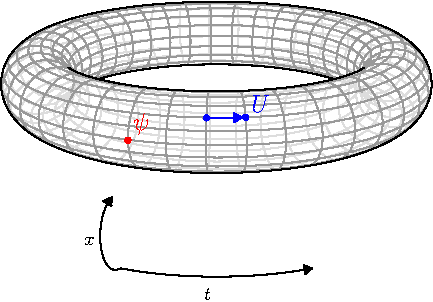
\includegraphics[width=0.8\linewidth]{figures/lattice_toroid_fields/lattice_toroid_fields.pdf}
\caption{ A $1+1$ dimensional toroid. When we discretize QCD onto a lattice the quark fields $\psi$ sit on the nodes of the lattice while the gluon fields live along the gauge links in the matrices $U$ which are elements of $SU(3)$. \label{fig::QCD_1p1_lattice_fields}}
\end{figure}
\clearpage
}

The discretization of the underlying field theory onto a lattice provides us a systematically improvable framework in which we can non-perturbatively evaluate correlation functions in the strongly coupled regime of QCD.



%%%%%%%%%%%%%%%%%%%%%%%%%%%%%%%%%%%%%%%%%%%%%%%%%%%%%%%%%
%%%%%%%%%%%%%%%%%%%%%%%%%%%%%%%%%%%%%%%%%%%%%%%%%%%%%%%%%
%%%%%%%%%%%%%%%%%%%%%%%%%%%%%%%%%%%%%%%%%%%%%%%%%%%%%%%%%

\section{Fermions in the Path Integral} \label{QCD::path_integral}

Having introduced the lattice discretization of the Euclidean path integral we now turn to an overview of methods which enable us to numerically estimate correlation functions. We look first to the fermion content of the path integral. Fermions anti-commute. In the language of operators this condition is imposed on the creation/annihilation field \emph{operators}. However, as mentioned previously, within the path integral formulation the fermions are replaced by \emph{numbers} which should be integrated over. In order to build in the anti-commutation under the path integral we represent the fermions by \emph{Grassman} numbers -- anti-commuting complex numbers.  A more detailed discussion of fermions and Grassman algebra can be found \appref{app::grassman}

The main result  is 
\begin{equation}
\label{eqn:fm_det}
\int d\eta d\bar{\xi}e^{\eta^TM\xi}  = \mathrm{det}(M),
\end{equation}
where $\eta$ and $\xi$ are vectors of Grassman numbers. 
 
Armed with this knowledge of Grassman integration, \eqnref{eqn:fm_det}, we now look to how we can use this formula to analytically integrate out the fermionic fields from the path integral. Recalling that we may specify any node on our lattice by a vector of integers, $\vec{n} = [n_x , n_y , n_z , n_t]$, and defining $\psi_n = \psi(a\vec{n})$, we may proceed to write the action in discretized form as 
\begin{equation*}
S[\psi,\bar{\psi},U] = S_{\mathrm{gauge}}[U]  + \sum_{n_1,n_2} \bar{\psi}_{n_1} M_{n_1,n_2}[U] \psi_{n_2} 
\end{equation*}
Where $M_{n_1,n_2}[U]$ represents the lattice discretization of the piece of the continuum Euclidean action appearing between the quark fields, $\left( \slashed{D} - m \right)$, $U$\footnote{$U$, the gauge field corresponds to a link variable. It is an element of $SU(3)$. There is a matrix, describing the gauge field, at each link on the lattice.} is the gauge field\footnote{The matrix, $M_{n_1,n_2}[U]$, contains dependence on the gauge field through the gauge covariant derivative appearing in the Lagrange density.}, and $S_\mathrm{gauge}[U]$ represents a lattice discretization of the gauge portion of the Lagrangian. The generating functional of the discretized Path Integral may be written as 
\begin{equation*}
\mathcal{Z}_{\mathrm{QCD}} = \int D[\psi,\bar{\psi},U] e^{-\bar{\psi}M[U]\psi \; - S_{\mathrm{gauge}}[U]}.
\end{equation*} 
Now using the integration formula for Grassman numbers (\eqnref{eqn:fm_det}) we see the fermion fields may be analytically integrated yielding 
\begin{equation*}
\mathcal{Z}_{\mathrm{QCD}} = \int D[U] e^{- S_{\mathrm{gauge}}[U]} \,\mathrm{det}(M[U]).
\end{equation*} 
This is an extremely powerful realization -- we do not need to represent \emph{anti-commuting complex numbers} on a computer. Further the preceding equation can be estimated via standard Markov-Chain Monte Carlo methods. 

%%%%%%%%%%%%%%%%%%%%%%%%%%%%%%%%%%%%%%%%%%%%%%%%%%%%%%%%%
%%%%%%%%%%%%%%%%%%%%%%%%%%%%%%%%%%%%%%%%%%%%%%%%%%%%%%%%%
%%%%%%%%%%%%%%%%%%%%%%%%%%%%%%%%%%%%%%%%%%%%%%%%%%%%%%%%% 
 
\subsection{Correlation Functions}

As mentioned previously, the fundamental theoretical objects of interest are correlation functions. For now it is useful to consider operators composed entirely of gauge links, we will lift this restriction after we have introduced the essential details related to the numeric estimation of correlation functions. Denoting our operator, composed only out of gauge links, as $\mathcal{O}_G$, such a correlation function takes the form
\begin{equation*}
\langle 0 | \hat{\mathcal{O}}_G  | 0 \rangle =  \frac{1}{\mathcal{Z}_{\mathrm{QCD}}}\int D[U] e^{-S_{\mathrm{gauge}}[U]} \,\mathrm{det}(M[U]) \,\mathcal{O}_G[U]. 
\end{equation*}

The simplest way one could estimate this correlation function is by drawing gauge configurations, at random, and then averaging over a finite but large number of configurations. For a lattice which contains $N$ sites along each direction there are $4N^4$ gauge links. Each link variable can be specified by eight real numbers\footnote{There are 8 generators of $SU(3)$, any element of the group can be written as $e^{i\theta_a t_a}$ where $\theta_a$ is a real number and $t_a$ is a generator. There is an implied summation on $a$.}, thus the parameter space of such a simulation is $32N^4$. Modern lattices contain roughly twenty nodes along any given direction; as a simple baseline we can consider a parameter space consisting of $512\times 10^4$ real numbers in the interval $[0,2\pi]$ -- one may expect that such a naive approach to estimating the correlation function would have poor convergence properties. 

Fortunately we can do much better. We do this by drawing the gauge configurations according to the probability density, 
\begin{equation}\label{eqn::MC_prob_dens}
P(U) = \frac{1}{\mathcal{Z}_{\mathrm{QCD}}}e^{-S_{\mathrm{gauge}}[U]} \,\mathrm{det}(M[U]).
\end{equation}
Integration methods of this form, drawing sample points according to some probability distribution, fall under the general class of algorithms called Markov Chain Monte Carlo methods\footnote{The Metropolis-Hastings algorithm is one such algorithm seen commonly in the context of numeric integration.}. 

Drawing from such a probability density also admits a classic interpretation of the integration path. Consider for a moment the principle of stationary action from Classical Mechanics. Minimization of the action corresponds roughly to a gauge field of maximum probability. Thus in an intuitive sense we can consider this formulation as sampling the Path Integral near the classical equations of motion. Those field configurations which minimize the action are exponentially preferred relative to those which are far from the classical solution\footnote{More correctly the probability is also proportional to $\det(M[U])$. The `action' in this case is then $e^{-S_G[U] + \ln(\det(M[U]))}$.}. 

By drawing a finite but large set of gauge configurations, $\{U_i\}$, according to the probability density in \eqnref{eqn::MC_prob_dens}, we can estimate the expectation value\footnote{This formulation also provides us with an estimate of the variance of the distribution.} as 
\begin{equation*}
\langle 0 | \hat{\mathcal{O}}_G  | 0 \rangle = \frac{1}{N} \sum_{\{U_i\}} \mathcal{O}_G[U_i].
\end{equation*}
More generally we will also be interested in computing correlation functions involving fermion fields. The numeric estimation of such correlation functions proceeds in the same manner and where the fermion fields are contracted together, the combination $\psi \bar{\psi}$ is replaced by the propagator, $M^{-1}[U]$. 
%Further details about Wick contractions and the evaluation of correlation functions featuring fermion fields can be found in \fcite{APPENDIX}.  

%%%%%%%%%%%%%%%%%%%%%%%%%%%%%%%%%%%%%%%%%%%%%%%%%%%%%%%%%
%%%%%%%%%%%%%%%%%%%%%%%%%%%%%%%%%%%%%%%%%%%%%%%%%%%%%%%%%
%%%%%%%%%%%%%%%%%%%%%%%%%%%%%%%%%%%%%%%%%%%%%%%%%%%%%%%%% 
 
\subsection{Symmetries and Intuition}

Having introduced the general technology used to sample correlation functions we now aim to build some intuition for the effect the lattice discretization has on our calculation. In particular we focus on the loss of rotational symmetry. When we consider QCD on a grid we do not have the ability to rotate by any infinitesimal angle as we do in the continuum. Rather, we can only perform rotations and reflections which leave the grid invariant. This means that the Hamiltonian, and thus the eigenstates, of our lattice discretized theory have a different symmetry group than their infinite volume continuum counterparts\footnote{Another way of saying this is that the operator which rotates by an infinitesimal angle does not commute with the lattice discretized Hamiltonian. The traditional set of quantum numbers must be replaced with a set that are good under cubic symmetry.}. 

\afterpage{
\begin{figure}[htbp]
\centering
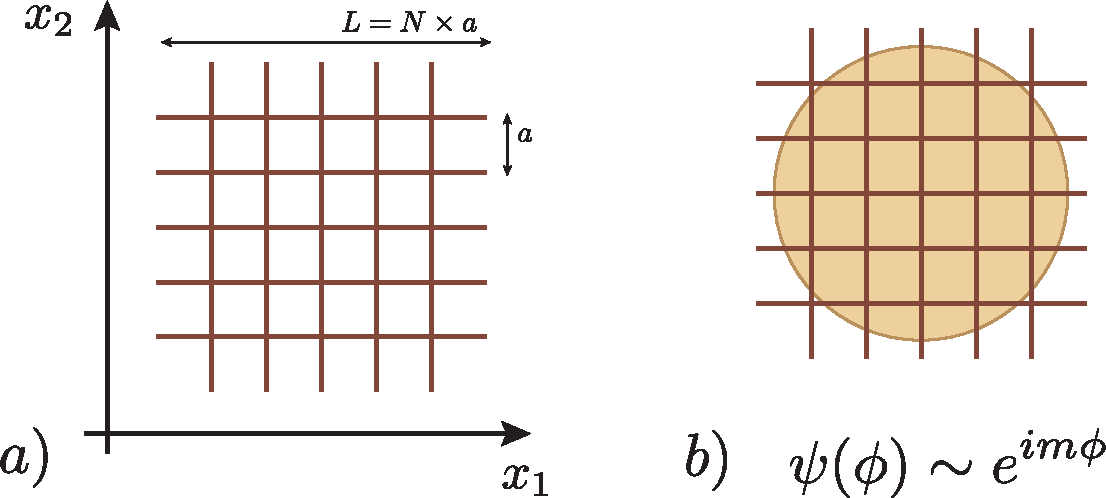
\includegraphics[width=0.7\linewidth]{figures/2DLattice/2dLatticeWavefuncs.pdf}
\caption{ A two dimensional lattice discretization. \label{fig::2DlatticeWavefuncs}}
\end{figure}
\clearpage
}

For example, if we think about a square discretization of a two dimensional theory, \figref{fig::2DlatticeWavefuncs}, we immediately realize that the square is only invariant under rotations by $\pi/2$. In a simple sense we have lost the ability to perform infinitesimal rotations which in turn mixes the angular momentum eigenstates.  For example, considering only rotations by $\pi/2$ we lose the ability to distinguish $m=0$ angular wave functions from $m=4$. 
 
This feature, reduced symmetry arising from the discretization, will reappear when we consider spectroscopy and matrix elements. We will find that particles transforming like spin-$J$ in the continuum are instead labeled by the irreducible representations of the symmetry group of the cube, multiple values of $J$ being present in any one irreducible representation. 






















































